\documentclass[final]{anthology-ch}

\usepackage{booktabs}
\usepackage{graphicx}
\usepackage{subcaption}
\usepackage{tikz}
\usepackage{color}
\usetikzlibrary{calc}
\usepackage{float}
\usetikzlibrary{shapes.geometric, arrows.meta, positioning}

\tikzset{
model/.style = {rectangle, draw=black, rounded corners, minimum width=2.5cm, minimum height=1cm, align=center, font=\small, fill=gray!5},
highlight/.style = {rectangle, draw=black, rounded corners, minimum width=2.5cm, minimum height=1cm, align=center, font=\small, fill=blue!10, very thick},
arrow/.style = {thick, ->, >=stealth},
fadedarrow/.style = {->, >=stealth, dashed, gray}
}

\title{Beyond Accuracy: Investigating Vision Model Perception on 19th-Century Decorative Arts}

\author[1]{Albina Toumarkine}[
]

\author[1,2]{Chahan Vidal-Gorène}[
orcid=0000-0003-1567-6508
]

\affiliation{1}{École nationale des chartes-PSL University, Paris}
\affiliation{2}{Centre Jean Mabillon, Paris}

\keywords{Islamic ornament, 19th-century ceramics, Unsupervised image analysis, Feature clustering, Interpretability, Vision transformers, Zero-shot learning}

\pubyear{2025}
\pubvolume{3}
\pagestart{1530}
\pageend{1548}
\conferencename{Computational Humanities Research 2025}
\conferenceeditors{Taylor Arnold, Margherita Fantoli, and Ruben Ros}
\doi{10.63744/k4Jy3Lr4rdK5}
\paperorder{97}
\addbibresource{bibliography.bib}

\begin{document}

\maketitle

\begin{abstract}

This paper examines how pretrained vision models perceive and organize a corpus of 19th-century decorative artefacts and printed materials. Using a zero-shot approach, we combine feature extraction, dimensionality reduction, and clustering to explore how convolutional and transformer architectures respond to historical visual material.
Two complementary experiments are presented: the first analyzes corpus-level organization through unsupervised clustering of VGG16 embeddings; the second investigates similarity retrieval from individual queries to compare model interpretability (VGG16, EfficientNet, ViT, DINOv2, and CLIP). By visualizing and aggregating activation maps, we discuss biases in how models attend to shape, ornament, and layout, often emphasizing background contrast or framing over meaningful decorative structure.  Rather than measuring accuracy, this study focuses on interpretability and bias, highlighting the challenges of adapting art-historical imagery to contemporary vision pipelines.
\end{abstract}

\section{Introduction}
\subsection{Background and related work in Art history} \label{sec:intro_details}
During the 19th century, the development of new industrial techniques led to a rapid expansion of applied and decorative arts, stimulating increased artistic, commercial, and institutional engagement with this field. Consequently, this period saw the establishment of new institutions dedicated to supporting the study and promotion of applied arts, reflecting the intersection of artistic practice and industrial production \cite{luneau_art_2013, froissart__1994}. Early examples include the South Kensington Museum in London (now the Victoria and Albert Museum) and the French Union Centrale des Arts Décoratifs (now the Musée des Arts Décoratifs in Paris).

Alongside this industrial and artistic development, a renewed European fascination with Islamic art began to emerge. Contemporary commentators frequently praised the quality and sophistication of Islamic ornamentation, often juxtaposing it with a perceived artistic decline in the industrializing West \cite{flood_islamic_2017}. This discourse positioned Islamic art as a valuable source of inspiration for European artists and manufacturers in search of aesthetic alternatives.

This enthusiasm for Islamic models manifested in a wide range of decorative objects that incorporated patterns and motifs drawn from Islamic arts, ranging from precise imitations to more freely adapted designs. Among the various media, ceramics were particularly influenced by Islamic art, often drawing directly on ceramic traditions—most notably Iznik ware, an Ottoman style renowned for its vivid colours, intricate floral and geometric motifs, and refined craftsmanship, mainly produced during the 16th and 17th centuries.

This artistic phenomenon has been widely studied through museum exhibitions, which bring together objects from different periods that are nonetheless closely connected, juxtaposing original artefacts from the Islamic world with the 19th-century decorative objects they inspired \cite{hagedorn_auf_1998,novakova_tulip_2003,labrusse_purs_2007,labrusse_islamophilies_2011,de_guise_inspired_2019}. Research arising from these exhibitions often highlights the emergence of new networks in the 19th century, connecting collectors, designers, industrialists, and scholars. It also raises important questions about how visual models circulated at a time when artefacts from the Islamic world were relatively rare and often held in private collections.

Printed materials have been proposed as a potential vector in these transmissions. They encompassed a wide range of formats, including journals specializing in the decorative arts and publications dedicated to Islamic art history. Pattern books, in particular, played a key role in the reproduction and adaptation of ornamental motifs \cite{froissart__2015}. Over time, designs drawn from Islamic art became increasingly present in these publications, with some volumes devoted entirely to ornamentation in Islamic arts.

Taken together, these developments reflect a proliferation of printed materials that greatly expanded the circulation of ornamental imagery, alongside the rise of serial production methods in the decorative arts. The scale and repetition introduced by these practices were inherently quantitative, revealing the limitations of isolated case studies and underscoring the relevance of large-scale analytical approaches for understanding how artistic forms spread.

\begin{figure}[t!]
\centering
\begin{subfigure}[b]{0.2\linewidth}
\includegraphics[width=\linewidth]{figures/Louvre_Iznik.JPG}
\caption{ }
\label{fig:iznik_bottle}
\end{subfigure}
\hspace{1em}
\begin{subfigure}[b]{0.2\linewidth}
\includegraphics[width=\linewidth]{figures/Deck_dish.jpg}
\caption{ }
\label{fig:samson_bottles}
\end{subfigure}
\hspace{1em}
\begin{subfigure}[b]{0.2\linewidth}
\includegraphics[width=\linewidth]{figures/beaumont_bassin.jpg}
\caption{ }
\label{fig:beaumont_bassin}
\end{subfigure}
\hspace{1em}
\begin{subfigure}[b]{0.2\linewidth}
\includegraphics[width=\linewidth]{figures/deck_bassin.jpg}
\caption{ }
\label{fig:deck_bassin}
\end{subfigure}
\caption{19th-Century European Reinterpretations of Islamic Art}
\caption*{\footnotesize (a) Iznik Dish, c. 1545, earthenware, Paris, Louvre, OA 6643. \\ (b) Théodore Deck, Dish, 1860-1870, earthenware, Guebwiller, Musée Théodore Deck, THD-993.3.10.\\ (c) Adalbert de Beaumont, Recueil de dessins pour l'art et l'industrie, Paris, Delâtre, 1859, pl. 54 \\ (d) Théodore Deck, Basin, 1863, earthenware, Paris, Musée des Arts Décoratifs, UC 515.}
\label{fig:19e-art-islam}

\end{figure}

To address this question, we combine large-scale image analysis with metadata-driven grouping to identify patterns of influence across visual corpora. A central objective is to assess the dissemination of ceramic designs derived from Islamic arts in 19th-century ceramic production, and to evaluate critically whether their influence has been as significant as traditionally assumed. Within a broader research framework, this project examines the dynamics of artistic transmission during the Industrial Era by modelling visual borrowing and transformation across a corpus of ceramic works and digitized printed materials. In doing so, it raises broader questions about cultural exchange, the diffusion of visual motifs, and the entanglement of art, industry, and printed media in the 19th century.

At a practical level, our aim is to identify connections between objects—here understood as instances of copying or reuse. To this end, we are conducting an extensive similarity search, which will serve as the basis for a network analysis. While human observers can readily perceive such visual similarities across decorative elements, these associations can be more difficult to detect computationally.

This paper presents the first phase of an ongoing research project, during which the question of interpretability emerged as a central concern. As we began applying pretrained computer vision models to an art-historical corpus of 19th-century ceramic artefacts and printed documents, we sought to understand how these models perceive and structure such material in a zero-shot setting. Beyond measuring performance, our aim is to reflect on what these models can meaningfully “see” in this context, as well as on the visual patterns, materials, and stylistic cues that they systematically fail to capture.

\begin{figure}[b!]
\centering
\includegraphics[height=100pt]{figures/Beaumont-Collinot_1880_035.jpg}
\includegraphics[height=100pt]{figures/Beaumont-Collinot_1880_021.jpg}
\includegraphics[height=100pt]{figures/PrissedAvennes_1877B_117.jpg}
\includegraphics[height=100pt]{figures/Jones_1856_199.jpg}
\includegraphics[height=100pt]{figures/Parvillee_1874_037.jpg}
\caption{Examples from the prints dataset, consisting of digitized 19th-century printed materials.}
\label{fig:corpus_docs}
\end{figure}

\subsection{Related work in Computer vision}
These initial objectives are grounded in the broader framework of distant viewing approaches \cite{arnold_distant_2019}. Tracking the circulations of visual forms presents significant methodological challenges that are increasingly addressed through computational means\cite{joyeux-prunel_visual_2019}.

Recent advances in computer vision have enabled large-scale visual analysis of cultural heritage objects, providing methods directly relevant to this study. For instance, Pondenkandath et al. (2021) developed CNN-based techniques for motif retrieval across different depictions of historical watermarks, demonstrating robust cross-depiction matching \cite{pondenkandath_cross-depicted_2020}. Zhao et al. (2023) applied deep learning to painted pottery, enabling similarity-based retrieval of motifs and visual clustering of stylistic traditions \cite{zhao_classification_2023}. Elgammal and Saleh (2015) proposed a network model to quantify originality and influence in art history, laying the groundwork for diffusion analysis \cite{elgammal_quantifying_2015}. Meinecke et al. (2024) addressed the challenge of inconsistent metadata in medieval image corpora using embedding-based visual analytics to support distant viewing approaches\cite{meinecke_is_2024}. Meyer et al. (2024) combined CLIP with object detection in museum collections to enable visual content-based search, highlighting the potential of vision–language models for multimodal exploration of decorative motifs \cite{meyer_algorithmic_2024}.

Several studies have also explored multimodal and similarity-based approaches to improve interpretability in artwork analysis. CLIP has been applied to the NoisyArt dataset to test zero-shot classification and retrieval capabilities, with GradCAM used to highlight the image regions most strongly associated with textual descriptions \cite{baldrati2022exploiting}. Similarly, the CLIP-Art model fine-tuned CLIP on the iMet collection through contrastive language–image pre-training to address fine-grained artwork classification and retrieval \cite{conde2021clip}. More recent transformer-based similarity approaches have emphasized attention-based embeddings to model cross-artwork visual affinities, underlining interpretability as a critical concern \cite{asperti2025does}. While these methods focus primarily on performance and multimodal generalization, our work emphasizes visual interpretability within a historical corpus rather than optimizing cross-domain retrieval accuracy.

\section{Methodology}

\subsection{Dataset}
The dataset comprises a heterogeneous corpus of historical printed materials and ceramic object photographs, assembled from a variety of institutional and online sources. While some images were gathered through automated harvesting methods (e.g., IIIF manifests), a substantial portion required manual selection to ensure alignment with the research scope. The final cleaned dataset contains 1,932 images for the print collection and 1,758 images for the object photographs.
For the experiments conducted here, we worked with a subset of 665 items in total, with 248 images consisting of digitized scans of historical pattern books. For volumes with broader coverage, only the pages or sections directly related to Islamic art were retained. These scans typically feature ornamental motifs in various formats: isolated figures, repeating patterns, or full decorative compositions (Figure ~\ref{fig:corpus_docs}).

The remaining 381 images are photographs of 19th-century ceramic objects, collected from museum and auction house websites. These images display variation in framing, lighting, and background treatment, and include both wide-angle and close-up views, capturing objects from multiple perspectives (e.g., frontal, oblique, and rear). No normalization or image pre-processing was applied (Figure ~\ref{fig:corpus_obj}).

\begin{figure}[t!]
\centering
\includegraphics[height=75pt]{figures/Bonhams_2023-12-19_71-01.jpg}
\includegraphics[height=75pt]{figures/Bonhams_2009-04-02_111-01.jpg}
\includegraphics[height=75pt]{figures/Sothebys_2022-10-26_152-03.jpg}
\includegraphics[height=75pt]{figures/museTheodoreDecketdespaysduFlorival_THD-DB-2002--1--113__-05.jpg}
\includegraphics[height=75pt]{figures/Bonhams_2025-06-12_32-02.jpg}
\caption{Examples from the artefacts dataset, comprising photographs of 19th-century ceramic objects.}
\label{fig:corpus_obj}
\end{figure}

Together, the two components form a visual corpus that reflects both historical reproduction (via print) and contemporary documentation (via photography). Each subset poses distinct challenges for computational analysis and requires tailored treatment within the data processing pipeline.

\begin{table}[h]
\centering
\begin{tabular}{cc}
\toprule
Data Category & Number of Images \\
\midrule
Scans of 19th-Century Prints & 248\\
Ceramic Artefact Photographs & 381 \\
\bottomrule
\end{tabular}
\caption{Overview of the two data categories used in the study.}
\label{tab:data_categories}
\end{table}

Working with such material exposes a fundamental tension between the art-historical notion of a \textit{corpus} and the computational notion of a \textit{dataset}. In art history, a \textit{corpus} is traditionally an assembled group of works selected to answer particular historical questions and shaped by critical judgment. The main criteria at stake are authorship, provenance, chronology, or context, guided by scholarly aims rather than by scale or standardization. On the other hand, a computer vision \textit{dataset} is constructed to meet computational requirements: it must contain large numbers of consistently formatted and annotated images suitable for algorithmic processing and statistical comparison. Treating art-historical images as datasets therefore raises important challenges: how to preserve meaning, context, and uncertainty within systems designed to favor uniformity and quantification, and, most importantly, how to critically examine the forms of attention, categorization, and visual logic that emerge when computer vision models analyze art in ways that diverge from human perception and historical understanding.

\subsection{Initial strategy and model selection}

Given the heterogeneity of the corpus and the absence of annotated data, understanding what a model “sees” in an image is rarely intuitive, and this opacity increases when the model is applied zero-shot to materials that differ substantially from its training data. Before evaluating whether pretrained models can extract art-historically relevant features, it is therefore essential to identify which visual attributes—though irrelevant to the research questions—might nonetheless dominate the model’s internal representations. This helps in designing more robust visual pipelines and preprocessing strategies. Thus, our initial objective was to evaluate the behavior of visual models without task-specific adaptation, since the corpus was relatively small and heterogeneous, computational resources were limited, and consistent labels or controlled conditions for meaningful fine-tuning were unavailable.

In a preliminary comparison, we tested several families of models — from multimodal vision–language architectures (OpenAI’s CLIP, BLIP, Microsoft’s Florence-2) to conventional convolutional backbones (VGG16). These experiments immediately highlighted the importance of interpretability: the groupings produced by vision–language models were difficult to interpret consistently, and Florence-based captioning followed by BERT embedding and PCA projection did not yield clusters that were visually or semantically coherent (see Appendix~\ref{fig:florence2_plot}). In contrast, convolutional models such as VGG16 displayed clearer internal structure in PCA space, with clusters that could be related to object shape, decorative density, or layout features. While these groupings were not always the most accurate in a strict quantitative sense, they proved more interpretable than the outputs of vision–language models.

Accordingly, we aimed to assess how pretrained models organize and interpret our dataset under zero-shot conditions and to identify configurations that produce interpretable structures rather than merely optimized ones. To this end, we designed two complementary experiments focusing on interpretability at different scales.

The first examines the global organization of the corpus through unsupervised clustering, revealing the visual regularities that emerge across the dataset as a whole. The second focuses on local relationships between individual images, exploring how specific features drive similarity and visual association within the learned representation space. Together, these experiments form a structured, multi-level approach that allows us to analyze how computer vision models, here VGG16, perceive and structure historical visual material, moving from corpus-level organization to image-level feature associations.

\subsection{Experiment 1 – Clustering of visual embeddings}

This first experiment applies a standard unsupervised pipeline combining VGG16 feature extraction, PCA dimensionality reduction, and K-Means clustering.

\begin{figure}[ht]
\centering
\resizebox{\textwidth}{!}{
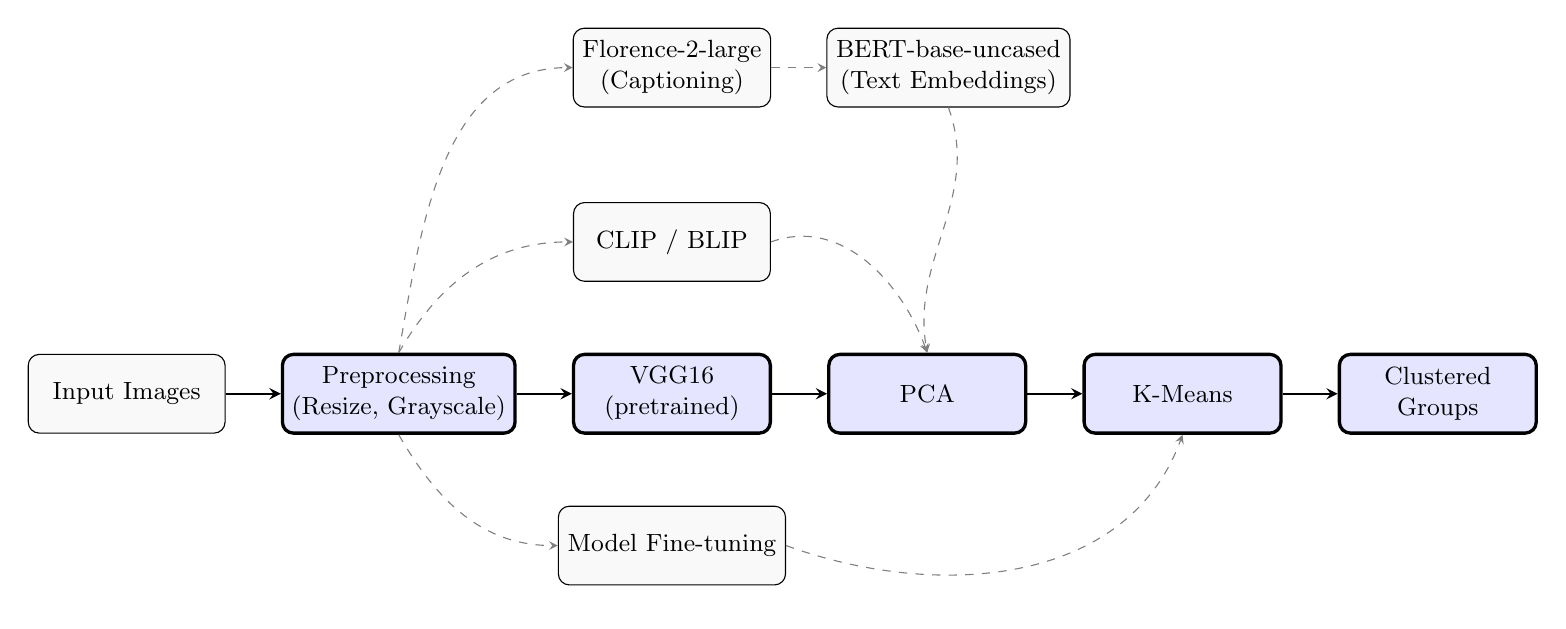
\begin{tikzpicture}[node distance=1.4cm and 0.7cm]

\node (input) [model] {Input Images};
\node (preprocess) [highlight, right=of input] {Preprocessing\\(Resize, Grayscale)};
\node (vgg) [highlight, right=of preprocess] {VGG16\\(pretrained)};
\node (pca) [highlight, right=of vgg] {PCA};
\node (kmeans) [highlight, right=of pca] {K-Means};
\node (output) [highlight, right=of kmeans] {Clustered\\Groups};

\draw [arrow] (input) -- (preprocess);
\draw [arrow] (preprocess) -- (vgg);
\draw [arrow] (vgg) -- (pca);
\draw [arrow] (pca) -- (kmeans);
\draw [arrow] (kmeans) -- (output);

\node (clip) [model, above=0.9cm of vgg] {CLIP / BLIP};
\draw [fadedarrow] (preprocess.north) to[out=60,in=180] (clip.west);
\draw [fadedarrow] (clip.east) to[out=20,in=110] (pca.north);

\node (finetune) [model, below=0.9cm of vgg] {Model Fine-tuning};
\draw [fadedarrow] (preprocess.south) to[out=-60,in=180] (finetune.west);
\draw [fadedarrow] (finetune.east) to[out=-20,in=-110] (kmeans.south);

\node (florence) [model, above=1.2cm of clip] {Florence-2-large\\(Captioning)};
\node (bert) [model, right=of florence] {BERT-base-uncased\\(Text Embeddings)};
\draw [fadedarrow] (preprocess.north) to[out=80,in=180] (florence.west);
\draw [fadedarrow] (florence.east) -- (bert.west);
\draw [fadedarrow] (bert.south) to[out=-70,in=100] (pca.north);

\end{tikzpicture}
}
\caption{Evaluated pipelines for unsupervised image grouping. All approaches start from a preprocessing stage (resizing, grayscale, channel duplication). The main path (highlighted) uses VGG16 with PCA and K-Means. Alternatives (gray) like Florence-based captioning with BERT, CLIP/BLIP, and fine-tuning were less effective or impractical for our corpus.}
\label{fig:modern_pipeline_updated}
\end{figure}

Each image is converted to grayscale, resized to 224 × 224 px, and processed through VGG16 (ImageNet weights, classification layers removed).
The resulting embeddings are projected with PCA to identify the main axes of visual variation, then grouped with K-Means to examine whether visually coherent clusters emerge, such as groupings based on shared shape, color, or ornament structure (Figures ~\ref{fig:plot_objannexe}, ~\ref{fig:plot_docs} and ~\ref{fig:plot_docs_crops}).

The analysis was conducted separately on the subset of object photographs (K = 7) and on the subset of print scans (K = 10). For the prints, the experiment was repeated with cropped borders for comparison. In both cases, the number of clusters was selected empirically through iterative inspection of clustering outcomes. While this approach provides an exploratory baseline, further refinement—such as using silhouette analysis or hierarchical evaluation metrics—will be required to stabilize K.

To examine the internal coherence of each cluster, we computed a mean feature heatmap by averaging the spatial activations of all cluster members within the last convolutional layer of VGG16. These visualizations help identify which regions of the artefacts most influence cluster assignments, indicating whether the grouping is driven by global form, surface texture, or decorative layout (Figures~\ref{fig:vgg-cluster-docs} and \ref{fig:vgg-cluster-obj}).

For each image $\mathbf{I}_i$, the pretrained network $f_{\theta}(\mathbf{I}_i)$ produces a feature vector
$\mathbf{z}_i \in \mathbb{R}^d$, which is projected with PCA and grouped using K-Means clustering.

To visualize how clusters are formed, we compute activation maps
$H_i = h_{\phi}(f_{\theta}, \mathbf{I}_i)$ by averaging the convolutional responses from the last spatial feature layer~$L$ of VGG16.
Formally, this can be expressed as:
\[
\bar{f}_{\theta}^{(L)}(\mathbf{I}_i) = \frac{1}{C} \sum_{c=1}^{C} f_{\theta,c}^{(L)}(\mathbf{I}_i),
\qquad
H_i = \frac{\bar{f}_{\theta}^{(L)}(\mathbf{I}_i)}
{\big\|\bar{f}_{\theta}^{(L)}(\mathbf{I}_i)\big\|},
\]
where $f_{\theta}^{(L)}(\mathbf{I}_i) \in \mathbb{R}^{C \times H_s \times W_s}$ corresponds to the activations from the last convolutional block of VGG16, with $C$ channels and spatial dimensions $(H_s, W_s)$.

For each cluster, a mean heatmap $\bar{H}_k$ is obtained by averaging the activation maps of all its member images:
\[
\bar{H}_k = \frac{1}{N_k} \sum_{i \in \mathcal{C}_k} H_i,
\]
where $\mathcal{C}_k$ is the set of images belonging to cluster $k$ and $N_k = |\mathcal{C}_k|$.
These averaged maps provide an aggregate view of the regions to which the model is most responsive within each group.
Random examples from each cluster are displayed alongside their corresponding mean heatmaps to illustrate the characteristic visual patterns captured by the model and to support the interpretation of its attention across clusters.

The combination of K-Means clustering with cluster-level mean heatmaps thus provides an interpretable baseline for observing how a generic CNN organizes form and ornament in 19th-century ceramic artefacts and printed materials.

\subsection{Experiment 2 - Similarity-based interpretability} \label{sec:querytask}

To complement the clustering-based analysis, this second experiment focuses on \textit{similarity retrieval from a single image query}.
While Experiment 1 examined the global structure of visual embeddings, here we analyze how models perceive similarity between individual images, an approach comparable to visual comparison in art history.

\paragraph{Objective.}
We aim to assess the interpretability of model-based similarities and compare their visual focus.
Each pretrained model retrieves the most similar artefacts for a given query image, based on its internal representation of form and texture.
For each retrieval, we compute a \textit{heatmap} showing which image zones contribute most to similarity, distinguishing meaningful decorative regions (motifs, texture) from irrelevant cues (contours, background, illumination).

\paragraph{Models and embeddings.}
Five pretrained architectures were evaluated, representing both convolutional and transformer-based paradigms:
\textbf{CNNs} (VGG16, EfficientNet-B7) and \textbf{Transformers} (ViT-Base (patch16-224), DINOv2-Base, and CLIP-ViT-B/32).
All were used in a zero-shot setting, operating solely from generic visual priors.
Each model transforms an image into a high-dimensional embedding $\mathbf{z}^{(m)} = f_{\theta_m}(\mathbf{I})$, indexed with FAISS using cosine similarity to retrieve the $k$ nearest neighbours (Figures ~\ref{fig:query_1_sim} and ~\ref{fig:query_2_sim}).

\paragraph{Retrieval and interpretability pipeline.}
For a query $\mathbf{I}_q$, its embedding $\mathbf{z}_q^{(m)}$ is compared to all others in the shared embedding space~$\mathcal{Z}$, and the top-$k$ most similar images are returned.
An activation map $H_m = g_{\phi_m}(\mathbf{I})$ highlights the regions most responsible for the similarity.
In convolutional models, $H_m$ averages final convolutional activations; in transformer models, it corresponds to mean attention weights per patch.
The most activated region $\mathbf{I}_{\text{crop}}^{(m)} = \arg\max H_m$ identifies the visual nucleus driving similarity.

Formally, this process can be expressed as:
\begin{equation*}
\bar{f}_{\theta_m}^{(L)}(\mathbf{I}) = \frac{1}{C} \sum_{c=1}^{C} f_{\theta_m,c}^{(L)}(\mathbf{I}),
\qquad
H_m = \frac{\bar{f}_{\theta_m}^{(L)}(\mathbf{I})}
{\big\|\bar{f}_{\theta_m}^{(L)}(\mathbf{I})\big\|},
\qquad
\mathbf{I}_{\text{crop}}^{(m)} = \arg\max H_m.
\end{equation*}
where $f_{\theta_m}$ denotes the pretrained vision model $m$ (e.g., VGG16, EfficientNet, ViT, DINOv2, CLIP),
and $f_{\theta_m}^{(L)}(\mathbf{I}) \in \mathbb{R}^{C \times H_s \times W_s}$ corresponds to the activations from its last spatial feature layer~$L$,
with $C$ channels and spatial dimensions $(H_s, W_s)$.
For convolutional networks, this layer corresponds to the final convolutional block;
for transformer-based architectures, it refers to the last attention block.

\paragraph{Dataset-level aggregation.}
Local activations $H_m(\mathbf{I}_i)$ are aggregated across the corpus to characterize each model’s global visual focus:
\[
\bar{H}_m = \frac{1}{N}\sum_{i=1}^{N} H_m(\mathbf{I}_i),
\]
where $N$ is the total number of images in the dataset.
For VGG, multi-layer activations (\texttt{block3–5}) are combined and normalized to integrate texture- and form-level features.
All activation vectors are then pooled, reduced with \textsc{UMAP}, and clustered using \textsc{HDBSCAN}, producing recurrent motif clusters that capture each model’s “visual signature” (see Figure~\ref{fig:query_pipeline_multimodel_refined}).

\begin{figure}[t!]
\centering
\resizebox{\textwidth}{!}{
\begin{tikzpicture}[node distance=2.6cm and 2.3cm, font=\small]

\node (img) [model, minimum width=3cm, minimum height=3cm, align=center] {
\textbf{Query Image}\\[-0.2em]
\includegraphics[width=2cm]{figures/Sothebys_2024-10-23_165_01.jpg}\\[-0.2em]
$\mathbf{I}_q$
};

\node (vgg) [highlight, right=of img, yshift=3cm, minimum width=4.2cm, align=center]
{VGG16\\$f_{\theta_1}(\mathbf{I}_q)$};
\node (vit) [highlight, right=of img, minimum width=4.2cm, align=center]
{ViT-Base\\$f_{\theta_2}(\mathbf{I}_q)$};
\node (clip) [highlight, right=of img, yshift=-3cm, minimum width=4.2cm, align=center]
{CLIP / DINOv2\\$f_{\theta_3}(\mathbf{I}_q)$};

\node (z1) [model, right=3.5cm of vgg, minimum width=1.3cm, minimum height=2.3cm, fill=blue!10] {};
\node (z2) [model, right=3.5cm of vit, minimum width=1.3cm, minimum height=2.3cm, fill=green!10] {};
\node (z3) [model, right=3.5cm of clip, minimum width=1.3cm, minimum height=2.3cm, fill=orange!10] {};
\node[above=0.1cm of z1, font=\scriptsize]{$\mathbf{z}_q^{(1)}$};
\node[above=0.1cm of z2, font=\scriptsize]{$\mathbf{z}_q^{(2)}$};
\node[above=0.1cm of z3, font=\scriptsize]{$\mathbf{z}_q^{(3)}$};

\node (latent) [highlight, right=7cm of vit, minimum width=7cm, minimum height=5cm, align=center, fill=gray!03] {};
\node[font=\small\bfseries] at ($(latent.north)+(0,-0.3)$) {Shared Embedding Space $\mathcal{Z}$};
\node[font=\scriptsize, below=0.1cm of latent.north, yshift=-0.25cm, text width=6cm, align=center]
{(FAISS cosine similarity and nearest-neighbour retrieval)};

\foreach \x/\y in {-1.2/0.8, -0.5/-0.5, 0.3/0.2, 0.9/-0.5, 1.3/0.7, 0.7/1.0, -0.9/0.2} {
\node[circle,fill=gray!45,inner sep=2pt] at ($(latent.center)+(\x*0.9,\y*0.9)$) {};
}

\node[circle,fill=blue!60,inner sep=2pt,label=left:{\scriptsize $\mathbf{z}_q^{(1)}$}] (lz1) at ($(latent.west)+(-0.8,1.3)$) {};
\node[circle,fill=green!60,inner sep=2pt,label=left:{\scriptsize $\mathbf{z}_q^{(2)}$}] (lz2) at ($(latent.west)+(-0.8,0.0)$) {};
\node[circle,fill=orange!70,inner sep=2pt,label=left:{\scriptsize $\mathbf{z}_q^{(3)}$}] (lz3) at ($(latent.west)+(-0.8,-1.3)$) {};
\node[circle,fill=red!70,inner sep=2.5pt,label=right:{\scriptsize $\mathbf{z}_1$}] (lzsim) at ($(latent.center)+(1.7,0.0)$) {};
\node[circle,fill=red!40,inner sep=2pt,label=right:{\scriptsize $\mathbf{z}_2$}] (lzsim2) at ($(lzsim)+(-0.7,0.7)$) {};
\node[circle,fill=red!25,inner sep=2pt,label=right:{\scriptsize $\mathbf{z}_3$}] (lzsim3) at ($(lzsim)+(-0.5,-0.7)$) {};

\draw[->,blue!70!black,thick] (z1.east) -- (lz1);
\draw[->,green!70!black,thick,dashed] (z2.east) -- (lz2);
\draw[->,orange!70!black,thick,dotted] (z3.east) -- (lz3);
\draw[->,blue!70!black,thick] (lz1) -- (lzsim);
\draw[->,green!70!black,thick,dashed] (lz2) -- (lzsim2);
\draw[->,orange!70!black,thick,dotted] (lz3) -- (lzsim3);

\node (retrieval) [highlight, right=7.4cm of latent, minimum width=4.5cm, align=center] {
\textbf{Top-$k$ Similar Images}\\[0.5em]
\includegraphics[height=2cm]{figures/Sothebys_2024-10-23_242_01.jpg}
\includegraphics[height=2cm]{figures/GazetteDrouot_2427983_01.jpg}\\[-0.2em]
$\{\mathbf{I}_1,\mathbf{I}_2,\mathbf{I}_3\}$\\
{\scriptsize Retrieved neighbours in embedding space}
};

\node (heatmap) [highlight, below=2.6cm of retrieval, minimum width=4.5cm, align=center] {
\textbf{Activation Heatmaps}\\[0.5em]
\includegraphics[width=3cm]{figures/heatmap_1.jpg}\\[-0.3em]
$H_m=g_{\phi_m}(\mathbf{I})$\\
{\scriptsize Regions most influencing similarity}
};

\node (crop) [highlight, below=2.6cm of heatmap, minimum width=4.5cm, align=center] {
\textbf{Most Activated Zone}\\[0.5em]
\includegraphics[height=2cm]{figures/crop1.jpg}
\includegraphics[height=2cm]{figures/crop2.jpg}
\includegraphics[height=2cm]{figures/crop3.jpg}\\[-0.3em]
$\mathbf{I}_{\text{crop}}^{(m)}=\arg\max H_m$
};

\node (compare) [highlight, left=3.4cm of heatmap, minimum width=6cm, align=center] {
\textbf{Cross-Model and Cross-Neighbors Interpretability Comparison}\\[0.5em]
\includegraphics[width=5cm]{figures/heatmap_comp.jpg}\\[-0.3em]
{\scriptsize VGG \hspace{1.5em} EfficientNet \hspace{1.5em} ViT \hspace{1.5em} CLIP}\\
{\scriptsize Comparison of attention patterns}
};

\node (globalagg) [highlight, below=2.6cm of compare, minimum width=6cm, align=center, fill=gray!05] {
\textbf{Dataset-Level Aggregation}\\[0.5em]
\includegraphics[width=3.2cm]{figures/vgg-multi-layer.jpg}\\[-0.3em]
$\bar{H}_m = \tfrac{1}{N}\sum_i H_m(\mathbf{I}_i)$\\
{\scriptsize Aggregation of activations across corpus}\\
{\scriptsize Model-level dominant crops and motifs}
};

\draw [arrow] (img) -- (vgg);
\draw [arrow] (img) -- (vit);
\draw [arrow] (img) -- (clip);
\draw [arrow] (vgg) -- (z1);
\draw [arrow] (vit) -- (z2);
\draw [arrow] (clip) -- (z3);
\draw [arrow, thick] (latent) -- node[above, font=\scriptsize] {retrieve top-$k$ neighbours} (retrieval);
\draw [arrow] (retrieval) -- (heatmap);
\draw [arrow] (heatmap) -- (crop);

\draw [arrow] (heatmap.west) -- ++(-1.6,0) |- (compare.east);

\draw [fadedarrow, dashed, gray]
([]latent.south west) to[out=280,in=180] (globalagg.west);

\draw [fadedarrow, dashed] (globalagg.east) -- (crop.west);

\end{tikzpicture}
}

\caption{
\textbf{Multi-model similarity interpretability pipeline.}
Each model retrieves top-$k$ similar images for a query $\mathbf{I}_q$.
Heatmaps $H_m$ highlight regions driving similarity, while the crops $\mathbf{I}_{\text{crop}}^{(m)}$ allow cross-model interpretability.
At the dataset level, activations from the embedding space are aggregated into $\bar{H}_m$, revealing global attention patterns and dominant motifs across the corpus. For clarity, EfficientNet is not shown in the diagram.
}

\label{fig:query_pipeline_multimodel_refined}
\end{figure}

\subsection{Results and discussion}

\paragraph{Evaluation protocol}
The pipeline was applied independently to the two subsets of our corpus: one comprising photographs of ceramic objects, and the other consisting of scans of printed materials. The goal in both cases was to organize the images into more coherent subgroups, facilitating further segmentation and cleaning.

Although the broader aim of the project is to investigate visual similarity between printed materials and objects, direct cross-dataset similarity scores between paper-based and ceramic images are generally low, reflecting inherent differences in medium, scale, and texture. By first concentrating on a single modality, we can identify which visual features and patterns the model prioritizes, providing insight to guide the design of subsequent cross-dataset similarity analyses.

\paragraph{Cluster structure (PCA)}
When clustered via K‑Means (K=7), the artefact embeddings split into visually coherent groups along two principal axes (see Figure~\ref{fig:plot_objannexe}). The first principal component (PC1) seems to correlate  with object shape: elongated, bottle‑form vessels exhibit high positive PC1 scores, whereas flat bowls and plates fall at the negative extreme. This suggests that VGG16 filters encode “verticality” versus “flatness” as a primary criterion of variation. The second component (PC2) aligns with decorative complexity: richly ornamented items—with dense floral or geometric motifs—occupy higher PC2 values, while more sparsely decorated or monochrome pieces load lower.

In the PCA plot of the full document images, several distinct visual groupings emerged (see Figure~\ref{fig:plot_docs}). The first principal component (PC1) captures large-scale layout differences: documents with heavy or full-page illustrations tend to lie on one end of the spectrum, while simpler documents—such as those showing isolated motifs or lighter printed layouts—are positioned toward the opposite side. The second component (PC2) appears to reflect a mixture of layout density and tonal contrast. For instance, documents with tightly packed visual information—such as grid-like arrangements of repeating motifs—cluster along one axis, while documents with broader white space or lower contrast occupy a more dispersed region.

However, closer inspection of the plot suggests that VGG16 may rely heavily on structural or framing features, such as dark zones in the background or shadowed page edges. These features, while visually consistent, are not semantically meaningful within the goals of this project, which seeks to distinguish actual content types (e.g., ornaments vs. object representations vs. architectural plans).

\paragraph{Mean activation maps per cluster}
The average activation heatmaps reveal a marked difference in the nature of the visual cues driving cluster formation in the two datasets. In the artefacts clusters, activations align with object contours and ornamented surfaces, indicating that clustering is driven by meaningful visual content such as shape and decorative density. In contrast, the document clusters show strong activation concentrated in the corners, suggesting that the model responds primarily to borders and binding shadows. Pages from the same volume frequently fall into the same cluster, not only because of similarities in their visual content, but also due to recurring layout and framing effects.

The impact of this reliance becomes clearer in the cropped-documents PCA–KMeans projection, where such peripheral cues were intentionally removed to evaluate their impact (see Figure~\ref{fig:plot_docs_crops}). Compared to the uncropped version, the overall structure of the PCA projection becomes more compact and internally coherent. Several clusters visible in the uncropped version collapse or reorganize, suggesting a stronger dependence on the central graphic content. Notably, in the cropped version, images representing isolated motifs and those containing continuous ornamental patterns begin to separate more cleanly, suggesting that the removal of background context has allowed the network’s representation to focus more on visual differences in the central subject matter. Additionally, certain architectural prints, which often had strong vertical lines or symmetrical structures, become less dominant in the representation space, further supporting the idea that the network was previously influenced by framing rather than semantic content.

\paragraph{Similarity-based interpretability}
The retrieval results in Figure~\ref{fig:query_pipeline_multimodel_refined} highlight distinct interpretability patterns across the evaluated models.
VGG16 provides the most spatially focused heatmaps, consistently emphasizing the central ornamental medallion and its surrounding radial motifs. The retrieved neighbours closely mirror these structural features, indicating that VGG16 relies heavily on mid-level form and texture.
EfficientNet also retrieves artefacts with comparable overall composition, but its activation maps differ in focus: they often place stronger weight on the border of the object and the circular framing elements.
In contrast, ViT displays broad and patchy attention spread. The activation patterns appear more evenly distributed across the surface of the object. While the retrieved images generally maintain comparable overall organization, the attention maps show less evidence of consistent focus on specific motifs, implying that the model may be capturing similarity in terms of broader shape or layout.
CLIP likewise retrieves artefacts that resemble the query in composition and palette, but its heatmaps more frequently highlight peripheral or low-texture regions. While it is difficult to attribute this behaviour to a single factor, it is consistent with broader representational tendencies observed in multimodal models, where similarity may be influenced jointly by local and global visual cues as well as broader stylistic or contextual associations.

\begin{figure}[t!]
\includegraphics[width=\linewidth]{figures/multi_heatmap.jpg}
\caption{Visualization of Experiment 2 results. For each model, the heatmaps show the query image (left) and its most similar retrieved artefacts. Warmer regions indicate areas most influential in the model’s perception of resemblance.}
\label{fig:heatmap_expe2}
\end{figure}

\paragraph{Metrics limitations}
Our evaluation is qualitative, as the dataset does not include ground truth labels or predefined categories that would allow the use of standard clustering metrics. We therefore assess cluster coherence by manually inspecting grouped images and analyzing their spatial distribution in the PCA projection.

\section{Conclusion}

This study applies a standard unsupervised pipeline—VGG16 feature extraction, PCA, and K-Means clustering—to photographs of 19th-century artefacts and digitized printed materials, without any task-specific training or fine-tuning. This setup reflects common constraints in digital humanities: limited data, heterogeneous image formats, and scarce resources for model adaptation.

Our observations refine prior insights on multimodal models applied to cultural heritage. While transformer-based pipelines demonstrate remarkable retrieval performance, their attention maps often reflect semantic or stylistic associations rather than strictly visual structures. In contrast, the convolutional hierarchy of VGG16 produces spatially coherent activations that align more closely with human perceptual logic—edges, contours, symmetry, and localized ornament. This contrast highlights that higher-performing multimodal transformers are not necessarily more interpretable for art-historical purposes.
Our results therefore reaffirm the analytical value of simpler convolutional architectures in interpretability-driven research, where the goal is not predictive accuracy but the legibility of visual correspondences.

A central aspect of this work is the adoption of a multi-scale interpretability strategy combining corpus-level grouping with spatial visualizations. At the corpus level, unsupervised clustering reveals how pretrained convolutional features organize the dataset into coherent groups, with mean cluster heatmaps highlighting recurrent regions of model sensitivity that are difficult to discern from individual images. At the image level, single-image heatmaps localize the specific ornamental details driving similarity judgments. This two-step approach forms a practical pipeline linking corpus-level structure to image-level visual evidence.

Even in this zero-shot setting, VGG16 captures some relevant visual properties, including shape, surface texture, and color distribution. While these attributes supported the emergence of partially coherent image clusters, they also revealed structural limitations. In particular, the model often prioritized superficial cues such as framing, background contrast, or page layout—features that do not always align with meaningful distinctions in the context of art historical analysis.

These findings underscore the gap between human visual reasoning and pretrained model behavior. Differences that are significant for researchers—such as decorative type, cultural reference, or motif composition—may be ignored by the model, while insignificant visual regularities are emphasized. Despite this, the interpretability of the representations and heatmaps proved useful for identifying biases and potential avenues for segmentation.

The lack of annotated labels prevents the use of conventional clustering metrics. As such, our evaluation remains qualitative, based on visual inspection of PCA distributions and intra-cluster coherence. This limits the reproducibility and validation of the results and remains a key methodological challenge to be addressed.

In future work, we aim to refine this approach by integrating visual and textual information. Although initial experiments combining Florence-2-generated captions with BERT embeddings did not yield meaningful structures, we believe that caption-based representations may offer complementary signals, particularly when dealing with human descriptions added in catalogs. Exploring such hybrid strategies could improve semantic grouping and help overcome current limitations in working with visually and semantically complex datasets.

Ultimately, while the digitized prints and photographs of ceramic artefacts are studied in our research as a corpus reflecting a single historical phenomenon, our experiments confirm the necessity of maintaining two distinct datasets for computational processing. Although this distinction may appear straightforward in our case, approaching heterogeneous and complex art-historical corpora from a model-interpretability perspective can help reveal subgroups \textit{as perceived by the model}, thereby guiding the steps—such as classification, normalization, or object detection—needed to make an art-historical corpus suitable for computational analysis.

\section*{Acknowledgements}

This study was conducted as part of the DH master’s program at École nationale des chartes–PSL. We thank Léa Saint-Raymond for her valuable feedback and suggestions. It also received support from the PSL Research University’s Major Research Program CultureLab, implemented by the ANR (reference ANR-10-IDEX-0001).

\section*{Data Availability}
Data samples were used exclusively for research purposes and cannot be shared, as they originate from sources such as museums, auction houses, and other cultural institutions.

\printbibliography

\appendix
\clearpage

\section{Appendix}
\label{appdx:first}

\begin{figure}[H]
\centering
\includegraphics[width=\linewidth]{figures/florence2_bert_pca.jpg}
\caption{PCA of BERT embeddings from Florence-2-large-generated captions.}
\label{fig:florence2_plot}
\end{figure}

\begin{figure}[H]
\centering
\begin{subfigure}[b]{0.9\linewidth}
\centering
\includegraphics[width=0.48\linewidth]{figures/pca_objets_img.jpg}
\includegraphics[width=0.42\linewidth]{figures/pca_objets.jpg}
\end{subfigure}
\caption{Visual Clustering of the Artefacts Dataset: K-Means Labels and PCA Image Projection}\label{fig:plot_objannexe}
\end{figure}

\begin{figure}[H]
\centering
\begin{subfigure}[b]{0.9\linewidth}
\centering
\includegraphics[width=0.48\linewidth]{figures/pca_docs.jpg}
\includegraphics[width=0.42\linewidth]{figures/pca_docs.jpg}
\end{subfigure}
\caption{Visual Clustering of the Prints Dataset: K-Means Labels and PCA Image Projection}\label{fig:plot_docs}
\end{figure}

\begin{figure}[H]
\centering

\begin{subfigure}[b]{0.9\linewidth}
\centering
\includegraphics[width=0.48\linewidth]{figures/pca_img_docs_crop.jpg}
\includegraphics[width=0.42\linewidth]{figures/pca_docs_crop.jpg}
\end{subfigure}
\caption{Visual Clustering of the Prints Dataset with Image Cropping: K-Means Labels and PCA Image Projection}\label{fig:plot_docs_crops}
\end{figure}

\begin{figure}[t!]
\centering
\includegraphics[width=0.85\textwidth]{figures/vgg-cluster-docs.jpg}
\caption{Cluster visualization based on PCA-projected VGG16 features, with mean activation heatmaps computed for each cluster. The first column shows the average heatmap of all items in the cluster, highlighting regions most attended by the model. The following five columns display randomly selected images from the cluster.
}
\label{fig:vgg-cluster-docs}
\end{figure}

\begin{figure}[t!]
\centering
\includegraphics[width=0.9\textwidth]{figures/vgg-cluster-obj.jpg}

\caption{Cluster visualization based on PCA-projected VGG16 features, with mean activation heatmaps computed for each cluster. The first column shows the average heatmap of all items in the cluster, highlighting regions most attended by the model. The following five columns display randomly selected images from the cluster.
}
\label{fig:vgg-cluster-obj}
\end{figure}

\begin{figure}[t!]
\includegraphics[width=\linewidth]{figures/query_1_vgg.png}
\includegraphics[width=\linewidth]{figures/query_1_efficient.png}
\includegraphics[width=\linewidth]{figures/query_1_vit.png}
\includegraphics[width=\linewidth]{figures/query_1_dino.png}
\includegraphics[width=\linewidth]{figures/query_1_clip.png}

\caption{
Example of similarity retrieval results for Experiment 2.
For each model, the first image (left) is the query, followed by the top-$k$ most similar artefacts retrieved in the embedding space.}
\label{fig:query_1_sim}
\end{figure}

\begin{figure}[t!]
\includegraphics[width=\linewidth]{figures/query_2_vgg.png}
\includegraphics[width=\linewidth]{figures/query_2_efficient.png}
\includegraphics[width=\linewidth]{figures/query_2_vit.png}
\includegraphics[width=\linewidth]{figures/query_2_dino.png}
\includegraphics[width=\linewidth]{figures/query_2_clip.png}

\caption{
Example of similarity retrieval results for Experiment 2.
For each model, the first image (left) is the query, followed by the top-$k$ most similar artefacts retrieved in the embedding space.}
\label{fig:query_2_sim}
\end{figure}

\end{document}